%==============================================================
%  EE201 -- Circuit Theory I
%  Lecture 12 : Mesh Current Analysis -- slides
%  M. Mert Ankaralı, METU EEE
%
%  Compile:  ./build.sh      (or: pdflatex EE201_Lecture_12_slides.tex, twice)
%  Same colour code as the handout:
%      charge = purple, current = blue, voltage = orange, power = green
%==============================================================
\documentclass[11pt,aspectratio=169]{beamer}

\usepackage[T1]{fontenc}
\usepackage[utf8]{inputenc}
\usepackage[english]{babel}
\usepackage{lmodern}
\usepackage{amsmath,amssymb}
\usepackage{booktabs}
\usepackage{array}
\usepackage{colortbl}
\usepackage{tikz}
\usepackage[american,siunitx]{circuitikz}
\usetikzlibrary{matrix,arrows.meta,positioning,calc,decorations.pathreplacing,decorations.pathmorphing,decorations.markings}
\usetikzlibrary{overlay-beamer-styles}

%-------------------- plain METU-flavoured theme --------------
\usetheme{default}
\usecolortheme{default}
\useinnertheme{rectangles}
\setbeamertemplate{navigation symbols}{}
\setbeamertemplate{itemize items}[square]
\setbeamerfont{frametitle}{size=\large,series=\bfseries}
\setbeamerfont{title}{size=\LARGE,series=\bfseries}

\definecolor{metured}{RGB}{155,27,48}
\definecolor{metugray}{RGB}{88,89,91}
\definecolor{metulight}{RGB}{243,240,241}
\definecolor{ccur}{RGB}{0,102,170}
\definecolor{cvolt}{RGB}{214,120,0}
\definecolor{cpow}{RGB}{23,128,74}
\definecolor{ccharge}{RGB}{124,60,160}
\definecolor{cflux}{RGB}{0,138,138}
\definecolor{copper}{RGB}{184,98,30}

\setbeamercolor{structure}{fg=metured}
\setbeamercolor{frametitle}{fg=metured,bg=}
\setbeamercolor{title}{fg=metured}
\setbeamercolor{normal text}{fg=black!88}
\setbeamercolor{block title}{fg=white,bg=metured}
\setbeamercolor{block body}{bg=metulight}
\setbeamercolor{alerted text}{fg=metured}

\setbeamertemplate{frametitle}{%
  \vspace{0.55em}%
  \usebeamerfont{frametitle}\usebeamercolor[fg]{frametitle}\insertframetitle\par
  \vspace{-0.2em}{\color{metured}\rule{\textwidth}{1pt}}\par\vspace{-0.2em}}

\setbeamertemplate{footline}{%
  \hbox{\begin{beamercolorbox}[wd=\paperwidth,ht=2.4ex,dp=1.4ex,leftskip=1.2em,rightskip=1.2em]{}%
  \tiny\color{metugray}\coursecode\ \textbar\ Lecture 12: Mesh Current Analysis
  \hfill \insertframenumber/\inserttotalframenumber
  \end{beamercolorbox}}}

%-------------------- macros ----------------------------------
\newcommand{\coursecode}{EE201}
\newcommand{\term}{Fall 2026--2027}
\newcommand{\Icol}[1]{\textcolor{ccur}{#1}}
\newcommand{\Vcol}[1]{\textcolor{cvolt}{#1}}
\newcommand{\Pcol}[1]{\textcolor{cpow}{#1}}
\newcommand{\Qcol}[1]{\textcolor{ccharge}{#1}}
\newcommand{\Fcol}[1]{\textcolor{cflux}{#1}}
\newcommand{\uni}[1]{\,\mathrm{#1}}
\newcommand{\A}{\uni{A}} \newcommand{\V}{\uni{V}}
\newcommand{\W}{\uni{W}} \newcommand{\J}{\uni{J}}
\newcommand{\Cb}{\uni{C}} \newcommand{\s}{\uni{s}}
\newcommand{\Wb}{\uni{Wb}} \newcommand{\Hy}{\uni{H}}
\newcommand{\Sie}{\uni{S}}


%  voltage sources: smaller + and - inside the circle, further apart
\ctikzset{bipoles/vsourceam/inner plus={\tiny$+$},
          bipoles/vsourceam/inner minus={\tiny$\vphantom{+}-$},
          bipoles/vsourceam/margin=0.85,
          bipoles/cvsourceam/inner plus={\tiny$+$},
          bipoles/cvsourceam/inner minus={\tiny$\vphantom{+}-$},
          bipoles/cvsourceam/margin=0.85}
\ctikzset{bipoles/length=0.9cm, label/align=straight,
          bipoles/generic/height=0.28, bipoles/generic/width=0.62}
\tikzset{
  iar/.style={-{Stealth[length=2.2mm]}, ccur, thick},
  glab/.style={font=\footnotesize, text=metured},
  ttl/.style={font=\scriptsize\bfseries, text=metugray},
  capn/.style={font=\scriptsize, text=metugray, align=center},
  pol/.style={font=\small, text=cvolt},
  nlab/.style={circle, draw=metured, text=metured, font=\scriptsize, inner sep=0.7pt},
  blab/.style={font=\footnotesize, text=black!80},
  gbr/.style={black!75, thick, postaction={decorate, decoration={markings,
      mark=at position 0.56 with {\arrow{Stealth[length=2.5mm]}}}}},
  hal/.style={draw=cpow!60, line width=6pt, opacity=0.35, line cap=round, line join=round},
  halo/.style={circle, fill=metured!16, minimum size=0.95cm},
  elem/.style={draw=metugray, thick, fill=metulight},
  bigarr/.style={-{Stealth[length=3mm]}, very thick, metugray},
}

%-------------------- Lecture 12 circuit macros ---------------
\newcommand{\ohm}{\,\Omega}
%  Colour-coded matrix entries: diagonal, off-diagonal, right side (#1 = colour of the right side)
\newcommand{\cbx}[2]{{\setlength{\fboxsep}{1.6pt}\colorbox{#1}{$\displaystyle #2\mathstrut$}}}
\newcommand{\dg}[1]{\cbx{cpow!16}{#1}}
\newcommand{\od}[1]{\cbx{metured!13}{#1}}
\newcommand{\chip}[1]{\textcolor{#1}{$\blacksquare$}}

%  An entry that appears on overlay #1, shown in red on that overlay
\newcommand{\zin}[2]{\uncover<#1->{\alt<#1>{{\textcolor{metured}{#2}}}{{#2}}}}
%  A highlighted matrix row entry: colour #1, content #2
\newcommand{\hrow}[2]{{\setlength{\fboxsep}{1.5pt}\colorbox{#1}{\makebox[2.1em]{$\mathstrut #2$}}}}
\newcommand{\yes}{\textcolor{cpow}{\checkmark}}
\newcommand{\no}{\textcolor{metured}{$\boldsymbol{\times}$}}
\newcommand{\e}[1]{\textcolor{cvolt}{e_{#1}}}
\newcommand{\im}[1]{\textcolor{ccur}{i_{M#1}}}
\newcommand{\nd}[1]{\tikz[baseline=(c.base)]\node[nlab](c){#1};}
\tikzset{mlabst/.style={draw=ccur, text=ccur, fill=white, rounded corners=1.5pt,
                        inner sep=1.2pt, font=\scriptsize\bfseries},
         smesh/.style={draw=metured, line width=5pt, opacity=0.28, line join=round}}
%  A boxed mesh number, for the text
\newcommand{\mlab}[1]{\tikz[baseline=(c.base)]\node[mlabst](c){#1};}
\newcommand{\smlab}{\tikz[baseline=(c.base)]\node[nlab](c){S};}
%  A clockwise mesh arrow at (#2,#3) with mesh number #4; optional radius #1
\newcommand{\meshcw}[4][0.36]{%
  \draw[ccur, thick, -{Stealth[length=2mm]}] ($(#2,#3)+(150:#1)$)
    arc[start angle=150, end angle=-150, radius=#1];
  \node[mlabst] at (#2,#3) {#4};}
%  A light disk behind a mesh, to point at it
\newcommand{\meshhalo}[3][0.62]{\fill[ccur!12] (#2,#3) circle (#1);}
\newcommand{\nodev}[3]{\fill (#1) circle (1.7pt) node[#2, inner sep=2pt, font=\small, text=cvolt] {#3};}
\newcommand{\gnd}[2]{\draw (#1,#2) -- ++(0,-0.2) node[ground] {};}

%  Examples 12.1 and 12.2: three meshes.
%  #1 = 0: v_s1 on the left (12.1);  1: i_s on the left (12.2).
%  #2 = 0: no mesh currents;  1: with the clockwise mesh currents.
\newcommand{\exM}[2]{%
  \ifnum#1=0
    \draw (0,2) to[american voltage source, l_=$\Vcol{v_{s1}}$] (0,0);
    \draw (7,0) to[american voltage source, l_=$\Vcol{v_{s2}}$] (7,2);
  \else
    \draw (0,0) to[american current source, l=$\Icol{i_s}$] (0,2);
    \draw (7,0) to[american voltage source, l_=$\Vcol{v_s}$] (7,2);
  \fi
  \draw (0,2) -- (0,3.5) to[R, l=$R_4$] (7,3.5) -- (7,2);
  \draw (0,2) to[R, l=$R_1$] (3.5,2) to[R, l=$R_3$] (7,2);
  \draw (3.5,2) to[R, l=$R_2$] (3.5,0);
  \draw (0,0) -- (7,0);
  \foreach \p in {(0,2),(3.5,2),(7,2),(3.5,0)} \fill \p circle (1.7pt);
  \ifnum#2>0
    \meshcw{1.6}{1.0}{1} \meshcw{5.5}{1.0}{2} \meshcw[0.33]{3.5}{2.8}{3}
  \fi}

%  Examples 12.3 and 12.4: two meshes with a current source between them.
%  #1 = 0: v_s on the right (12.3);  1: the CCVS r_m i_x on the right (12.4).
%  #2 = 0: no mesh currents;  1: mesh currents;  2: mesh currents and the supermesh;
%       3: mesh currents and the voltage v of the current source (Method I).
\newcommand{\exN}[2]{%
  \draw (0,0) to[R, l=$R_1$] (0,2.2) to[R, l=$R_2$] (3,2.2) to[R, l=$R_3$] (6,2.2);
  \draw (3,2.2) to[american current source, l=$\Icol{i_s}$] (3,0);
  \ifnum#1=0
    \draw (6,2.2) to[american voltage source, l=$\Vcol{v_s}$] (6,0);
  \else
    \draw (6,2.2) to[american controlled voltage source, l=$\Vcol{r_m i_x}$] (6,0);
    \draw[iar] (-0.28,1.62) -- (-0.28,2.12); \node[font=\small, text=ccur] at (-0.58,1.9) {$i_x$};
  \fi
  \draw (0,0) -- (6,0);
  \foreach \p in {(3,2.2),(3,0)} \fill \p circle (1.7pt);
  \ifnum#2>0 \meshcw{1.45}{1.1}{1} \meshcw{4.75}{1.1}{2} \fi
  \ifnum#2=2
    \draw[smesh] (0,0) -- (0,2.2) -- (6,2.2) -- (6,0) -- cycle;
    \node[nlab] at (0.55,0.38) {S};
  \fi
  \ifnum#2=3
    \node[pol] at (2.62,1.75) {$+$}; \node[pol] at (2.62,0.45) {$-$};
    \node[font=\small, text=cvolt] at (2.45,1.1) {$v$};
  \fi}

%  Example 12.5: a dependent current source 3 v_x on the top branch.
%  #1 = 0: bare;  1: mesh currents;  2: mesh currents and the supermesh of meshes 1 and 2;
%       3: node voltages (ground at the right node).
\newcommand{\exP}[1]{%
  \draw (7.2,3.8) to[american controlled current source, l_=$\Icol{3\,v_x}$] (0,3.8);
  \draw (0,3.8) -- (0,2); \draw (7.2,3.8) -- (7.2,2);
  \draw (0,2) to[R, l=$4\ohm$] (3.6,2) to[american voltage source, l=$\Vcol{12\V}$] (7.2,2);
  \draw (0,0) to[R, l=$2\ohm$] (0,2);
  \draw (3.6,0) to[american current source, l_=$\Icol{2\A}$] (3.6,2);
  \draw (7.2,2) to[R, l=$6\ohm$] (7.2,0);
  \draw (0,0) -- (7.2,0);
  \foreach \p in {(0,2),(3.6,2),(7.2,2),(3.6,0)} \fill \p circle (1.7pt);
  \node[pol] at (0.35,1.6) {$+$}; \node[pol] at (0.35,0.4) {$-$};
  \node[font=\small, text=cvolt] at (0.5,1.0) {$v_x$};
  \draw[iar] (1.45,1.72) -- (2.15,1.72); \node[font=\small, text=ccur] at (2.4,1.72) {$i$};
  \ifnum#1>0 \ifnum#1<3
    \meshcw{1.65}{0.85}{1} \meshcw{5.7}{0.9}{2} \meshcw[0.32]{3.6}{2.95}{3}
  \fi\fi
  \ifnum#1=2
    \draw[smesh] (0,0) -- (0,2) -- (7.2,2) -- (7.2,0) -- cycle;
    \node[nlab] at (3.1,0.35) {S};
  \fi
  \ifnum#1=3
    \node[font=\small, text=cvolt, anchor=south east] at (-0.05,2.05) {$e_1$};
    \node[font=\small, text=cvolt, anchor=north] at (3.6,-0.1) {$e_2$};
    \draw (7.2,3.8) -- (7.8,3.8) -- (7.8,3.6) node[ground] {};
  \fi}

%  Graph branch from #2 to #3, label #5 on side #4 (angle), optional colour #1
\newcommand{\gbranch}[5][black!75]{%
  \draw[gbr, #1] (#2) -- (#3);
  \node[blab, text=#1] at ($(#2)!0.5!(#3)!0.3cm!#4:(#3)$) {#5};}
%  The graph of Example 12.1: branches 1-4 the resistors R1-R4, 5 and 6 the sources v_s1, v_s2.
%  #1 = 0: graph only;  1: with the clockwise meshes.
\newcommand{\exMgraph}[1]{%
  \coordinate (ga) at (0,1.5); \coordinate (gb) at (2.2,1.5);
  \coordinate (gc) at (4.4,1.5); \coordinate (gd) at (2.2,0);
  \gbranch{ga}{gb}{90}{1}
  \gbranch{gb}{gd}{0}{2}
  \gbranch{gb}{gc}{90}{3}
  \draw[gbr] (ga) to[bend left=50] (gc); \node[blab] at (2.2,2.72) {4};
  \draw[gbr, cvolt] (ga) to[bend right=40] (gd); \node[blab, text=cvolt] at (0.42,0.32) {5};
  \draw[gbr, cvolt] (gd) to[bend right=40] (gc); \node[blab, text=cvolt] at (3.98,0.32) {6};
  \foreach \k in {a,b,c,d} \fill[metured] (g\k) circle (2.2pt);
  \ifnum#1>0
    \meshcw[0.27]{1.3}{0.82}{1} \meshcw[0.27]{3.1}{0.82}{2} \meshcw[0.27]{2.2}{2.08}{3}
  \fi}
%  A mesh matrix with mesh labels on the left and branch numbers on top.
%  #1 name, #2 number of columns, #3 number of rows, #4 rows (entries separated by \&), #5 extra TikZ
\newcommand{\meshmat}[5]{%
  \begin{tikzpicture}[baseline={([yshift=-0.6ex]#1.center)}]
    \matrix (#1) [matrix of math nodes, ampersand replacement=\&,
                  left delimiter={[}, right delimiter={]}, inner sep=1pt,
                  column sep=0.45em,
                  nodes={text width=1.35em, align=right, minimum height=1.25em,
                         inner sep=1pt}] {#4};
    \foreach \j in {1,...,#2}
      \node[font=\scriptsize, text=metugray, anchor=south east, inner sep=1pt]
        at ([yshift=2pt]#1-1-\j.north east) {\j};
    \foreach \i in {1,...,#3}
      \node[mlabst, left=11pt] at (#1.west |- #1-\i-1) {\i};
    #5
  \end{tikzpicture}}
%  \exMmatN{k}: the mesh matrix M of Example 12.1 with its first k rows filled in;
%  k = 4 adds the M_R / M_S boxes
\newcommand{\phrow}{\phantom{0} \& \phantom{0} \& \phantom{0} \& \phantom{0} \& \phantom{0} \& \phantom{0}}
\newcommand{\exMmatN}[1]{%
  \ifnum#1>0 \def\rowA{1 \& 1 \& 0 \& 0 \& \textcolor{cvolt}{-1} \& \textcolor{cvolt}{0}}%
  \else\let\rowA\phrow\fi
  \ifnum#1>1 \def\rowB{0 \& -1 \& 1 \& 0 \& \textcolor{cvolt}{0} \& \textcolor{cvolt}{-1}}%
  \else\let\rowB\phrow\fi
  \ifnum#1>2 \def\rowC{-1 \& 0 \& -1 \& 1 \& \textcolor{cvolt}{0} \& \textcolor{cvolt}{0}}%
  \else\let\rowC\phrow\fi
  \meshmat{MM}{6}{3}{\rowA\\ \rowB\\ \rowC\\}{%
    \ifnum#1>3
    \draw[metugray, thick, rounded corners=2pt]
      ([xshift=-2pt, yshift=1pt]MM-1-1.north west) rectangle ([xshift=2pt, yshift=-1pt]MM-3-4.south east);
    \draw[cvolt, thick, rounded corners=2pt]
      ([xshift=-2pt, yshift=1pt]MM-1-5.north west) rectangle ([xshift=2pt, yshift=-1pt]MM-3-6.south east);
    \node[font=\small, text=metugray, below=3pt] at ($(MM-3-1.south)!0.5!(MM-3-4.south)$) {$M_R$: resistors};
    \node[font=\small, text=cvolt, below=3pt] at ($(MM-3-5.south)!0.5!(MM-3-6.south)$) {$M_S$: sources};
    \else
    \node[font=\small, below=3pt] at ($(MM-3-1.south)!0.5!(MM-3-4.south)$) {\phantom{$M_R$: resistors}};
    \fi}}
\newcommand{\exMmat}{\exMmatN{4}}
\title{Lecture 12: Mesh Current Analysis}
\subtitle{EE201 -- Circuit Theory I}
\author{M. Mert Ankaralı}
\institute{\small Department of Electrical and Electronics Engineering\\
           Middle East Technical University}
\date{}

%  Roadmap icons, one per stop (1-7)
\newcommand{\rmicon}[1]{%
  \ifcase#1\or
    \draw (-1.1,-0.6) to[american voltage source] (-1.1,0.6) to[R] (1.1,0.6) to[R] (1.1,-0.6) -- (-1.1,-0.6);
    \draw[ccur, line width=1.6pt, -{Stealth[length=1.7mm, width=1.7mm]}] (0,0)+(150:0.36) arc[start angle=150, end angle=-150, radius=0.36];
  \or
    \node[font=\LARGE] at (0,0) {$\begin{bmatrix} \ast & \ast\\ \ast & \ast \end{bmatrix}$};
  \or
    \draw (-1.1,-0.6) to[american current source] (-1.1,0.6) to[R] (1.1,0.6) to[R] (1.1,-0.6) -- (-1.1,-0.6);
  \or
    \draw (-1.6,-0.6) to[R] (-1.6,0.6) -- (1.6,0.6) to[R] (1.6,-0.6) -- (-1.6,-0.6);
    \draw (0,0.6) to[american current source] (0,-0.6);
  \or
    \draw[metured, line width=6pt, opacity=0.3] (-1.6,-0.6) rectangle (1.6,0.6);
    \draw (-1.6,-0.6) to[R] (-1.6,0.6) -- (1.6,0.6) to[R] (1.6,-0.6) -- (-1.6,-0.6);
    \draw (0,0.6) to[american current source] (0,-0.6);
  \or
    \draw (-1.5,0) -- (-0.9,0) to[american controlled current source] (0.9,0) -- (1.5,0);
  \or
    \fill[cvolt] (-0.9,0) circle (6pt);
    \node[font=\LARGE\bfseries] at (0,0) {?};
    \draw[ccur, line width=1.6pt, -{Stealth[length=1.7mm, width=1.7mm]}] (0.95,0)+(150:0.42) arc[start angle=150, end angle=-150, radius=0.42];
  \fi}
%  Roadmap: four stations on a road; each station adds a new kind of source.
%  Stops 1-7 are the sub-items: station of stop k = \rmst{k}
\newcommand{\rmst}[1]{\ifcase#1\or1\or1\or2\or2\or2\or3\or4\fi}
%  #1 station, #2 x, #3 title, #4 icon number
\newcommand{\rmstation}[4]{%
  \ifnum#1<\rmS\relax
    \node[circle, fill=cpow, text=white, inner sep=0pt, minimum size=5.4mm, font=\scriptsize\bfseries] at (#2,0) {\checkmark};
    \node[text=black!40, font=\bfseries] at (#2,0.62) {#3};
  \else\ifnum#1=\rmS\relax
    \node[circle, fill=metured, text=white, inner sep=0pt, minimum size=6.2mm, font=\small\bfseries] at (#2,0) {#1};
    \node[text=metured, font=\bfseries] at (#2,0.62) {#3};
  \else
    \node[circle, draw=metugray, fill=white, text=metugray, inner sep=0pt, minimum size=5.4mm, font=\scriptsize\bfseries] at (#2,0) {#1};
    \node[font=\bfseries] at (#2,0.62) {#3};
  \fi\fi
  \begin{scope}[shift={(#2,1.45)}, scale=0.42, transform shape]
    \ifnum#1>\rmS\relax\begin{scope}[opacity=0.5]\rmicon{#4}\end{scope}\else\rmicon{#4}\fi
  \end{scope}}
%  #1 first stop, #2 last stop covered by this item, #3 x, #4 y, #5 text
\newcommand{\rmsub}[5]{%
  \ifnum#2<\rmcur\relax
    \node[text width=3.05cm, align=center, font=\small, text=black!40] at (#3,#4) {#5\ \textcolor{cpow}{\checkmark}};
  \else\ifnum#1>\rmcur\relax
    \node[text width=3.05cm, align=center, font=\small] at (#3,#4) {#5};
  \else
    \node[text width=3.05cm, align=center, font=\small\bfseries, text=metured,
          draw=metured, rounded corners=2pt, inner sep=2pt] at (#3,#4) {#5};
  \fi\fi}
\newcommand{\roadmapframe}[1]{%
  \begin{frame}{Roadmap}
    \def\rmcur{#1}\edef\rmS{\rmst{#1}}%
    \vfill
    \centering
    \begin{tikzpicture}
      \draw[metugray!45, line width=3pt, -{Stealth[length=2.6mm, width=3.2mm]}] (0,0) -- (13.3,0);
      \rmstation{1}{1.75}{Voltage sources}{1}
      \rmstation{2}{5.0}{Current sources}{4}
      \rmstation{3}{8.45}{Dependent sources}{6}
      \rmstation{4}{11.65}{Node or mesh?}{7}
      \rmsub{1}{1}{1.75}{-0.8}{the procedure, on an example}
      \rmsub{2}{2}{1.75}{-1.75}{matrix form}
      \rmsub{3}{3}{5.0}{-0.8}{on one mesh only}
      \rmsub{4}{5}{5.0}{-1.75}{between two meshes}
      \rmsub{6}{6}{8.45}{-0.8}{a dependent current source}
      \rmsub{7}{7}{11.65}{-0.8}{the same circuit both ways}
    \end{tikzpicture}
    \vfill
    \mbox{}
    \vfill
  \end{frame}}

\begin{document}

%--------------------------------------------------------------
\begin{frame}[plain]
  \titlepage
  \vspace{-1.2em}
  \begin{center}\scriptsize\color{metugray}
    \Icol{$\blacksquare$}~current, mesh current \mlab{1} \quad \Vcol{$\blacksquare$}~voltage \quad
    \textcolor{metured}{$\blacksquare$}~supermesh
  \end{center}
\end{frame}

%--------------------------------------------------------------
\begin{frame}{Review: node voltage analysis}
  \begin{columns}[t,onlytextwidth]
    \begin{column}{0.47\textwidth}
      \begin{block}{The procedure}
        \begin{itemize}\itemsep3pt
          \item Ground; node voltages $\Vcol{\mathbf{e}}$
          \item KVL automatic: $\Vcol{\mathbf{v}} = A^T\Vcol{\mathbf{e}}$
          \item KCL at non-ground nodes
          \item $Y_n\Vcol{\mathbf{e}} = \Icol{\mathbf{i}_n}$
        \end{itemize}
      \end{block}
    \end{column}
    \begin{column}{0.47\textwidth}
      \onslide<2->{%
      \begin{block}{Voltage sources}
        \begin{itemize}\itemsep3pt
          \item To the ground: $\e{k}$ known
          \item Between two nodes: supernode
          \item Dependent: one more constraint
        \end{itemize}
      \end{block}}
    \end{column}
  \end{columns}
  \vfill
  \onslide<3->{%
  \begin{center}
    \alert{KVL} automatic, we write \alert{KCL}\\[4pt]
    \onslide<4->{The opposite?}
  \end{center}}
  \vfill
\end{frame}

%--------------------------------------------------------------
\begin{frame}{Motivation}
  \vspace{2pt}
  \begin{columns}[t,onlytextwidth]
    \begin{column}{0.47\textwidth}
      \begin{block}{Node voltages}
        \begin{itemize}\itemsep5pt
          \item Unknowns: $n - 1$ node voltages
          \item KVL automatic
          \item Write KCL
        \end{itemize}
      \end{block}
    \end{column}
    \begin{column}{0.47\textwidth}
      \onslide<2->{%
      \begin{block}{Mesh currents}
        \begin{itemize}\itemsep5pt
          \item Unknowns: $\ell = b - n + 1$ mesh currents
          \item<3-> KCL automatic: $\Icol{\mathbf{i}} = M^T\Icol{\mathbf{i}_M}$
          \item<4-> Write KVL
          \item<5-> Needs a \alert{planar} circuit
        \end{itemize}
      \end{block}}
    \end{column}
  \end{columns}
  \vfill
\end{frame}

%==============================================================
\roadmapframe{1}

%--------------------------------------------------------------
\begin{frame}{Example 12.1: mesh current analysis step by step}
  \begin{center}
    {\small For now: only \alert{resistors} and \alert{independent voltage sources}}
  \end{center}
  \begin{columns}[c,onlytextwidth]
    \begin{column}{0.55\textwidth}
      \centering
      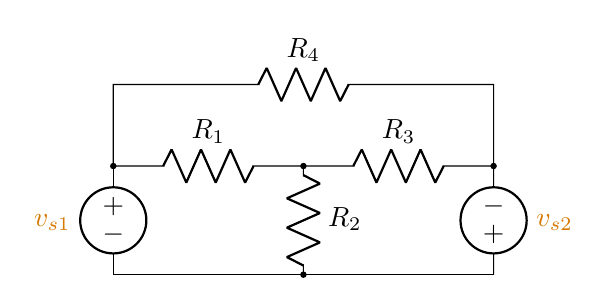
\begin{tikzpicture}[scale=0.69]
        \exM{0}{0}
      \end{tikzpicture}
    \end{column}
    \begin{column}{0.41\textwidth}
      \textbf{Goal:} every branch current and voltage\\[12pt]
      \textbf{Four steps:}
      \begin{enumerate}\itemsep4pt
        \item Find the inner meshes
        \item Assign the mesh currents
        \item Resistor voltages with mesh currents
        \item KVL around every inner mesh
      \end{enumerate}
    \end{column}
  \end{columns}
\end{frame}

%--------------------------------------------------------------
\begin{frame}{Step 1: find the inner meshes}
  \begin{columns}[c,onlytextwidth]
    \begin{column}{0.55\textwidth}
      \centering
      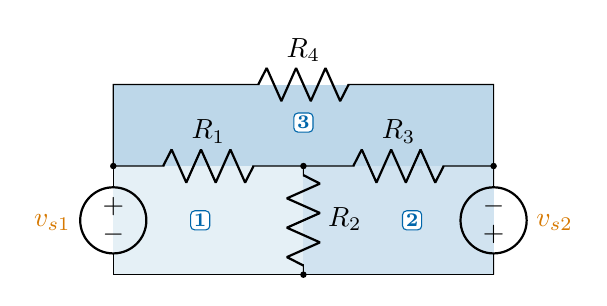
\begin{tikzpicture}[scale=0.69]
        \only<2->{%
          \fill[ccur!10] (0,0) rectangle (3.5,2); \fill[ccur!18] (3.5,0) rectangle (7,2);
          \fill[ccur!26] (0,2) rectangle (7,3.5);
          \node[mlabst] at (1.6,1.0) {1}; \node[mlabst] at (5.5,1.0) {2};
          \node[mlabst] at (3.5,2.8) {3};}
        \exM{0}{0}
      \end{tikzpicture}
    \end{column}
    \begin{column}{0.41\textwidth}
      \alert{Planar}: no crossing branches\\[12pt]
      \onslide<2->{%
      \alert{Inner meshes}: the windows\\[12pt]}
      \onslide<3->{%
      $\ell = b - n + 1 = 6 - 4 + 1 = 3$}
    \end{column}
  \end{columns}
\end{frame}

%--------------------------------------------------------------
\begin{frame}{Step 2: assign the mesh currents}
  \begin{columns}[c,onlytextwidth]
    \begin{column}{0.55\textwidth}
      \centering
      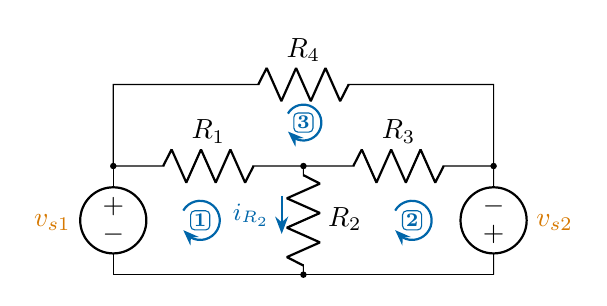
\begin{tikzpicture}[scale=0.69]
        \exM{0}{1}
        \only<2->{\draw[iar] (3.1,1.45) -- (3.1,0.75);
          \node[font=\small, text=ccur, anchor=east] at (3.05,1.1) {$i_{R_2}$};}
      \end{tikzpicture}
    \end{column}
    \begin{column}{0.41\textwidth}
      Unknowns, clockwise: \ $\im{1}$, $\im{2}$, $\im{3}$\\[12pt]
      \onslide<2->{%
      $\Icol{i_{R_2}} = \im{1} - \im{2}$\\[12pt]}
      \onslide<3->{%
      KCL holds \alert{automatically}}
    \end{column}
  \end{columns}
\end{frame}

%--------------------------------------------------------------
\begin{frame}{Step 3: write the resistor voltages with mesh currents}
  \begin{columns}[c,onlytextwidth]
    \begin{column}{0.55\textwidth}
      \centering
      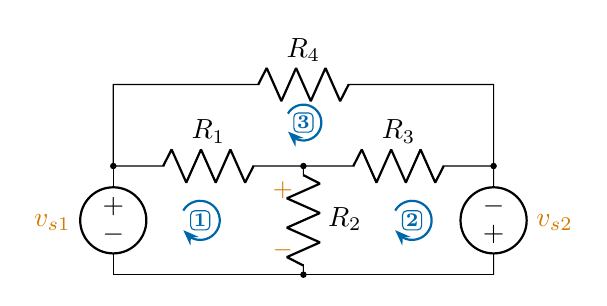
\begin{tikzpicture}[scale=0.69]
        \exM{0}{1}
        \node[pol] at (3.12,1.55) {$+$}; \node[pol] at (3.12,0.45) {$-$};
      \end{tikzpicture}
    \end{column}
    \begin{column}{0.41\textwidth}
      $R_2$, along mesh 1:\\[3pt]
      $\Vcol{v} = R_2(\im{1} - \im{2})$\\[12pt]
      $R_4$: \ $\Vcol{v} = R_4\,\im{3}$\\[12pt]
      \fbox{\ $R\,(\text{own} - \text{other})$\ }
    \end{column}
  \end{columns}
\end{frame}

%--------------------------------------------------------------
\begin{frame}{Step 4: KVL around every inner mesh}
  \begin{columns}[c,onlytextwidth]
    \begin{column}{0.47\textwidth}
      \centering
      \begin{tikzpicture}[scale=0.64]
        \only<1>{\fill[ccur!14] (0,0) rectangle (3.5,2);}
        \only<2>{\fill[ccur!14] (3.5,0) rectangle (7,2);}
        \only<3>{\fill[ccur!14] (0,2) rectangle (7,3.5);}
        \exM{0}{1}
      \end{tikzpicture}
    \end{column}
    \begin{column}{0.5\textwidth}
      \small
      \textbf{Mesh 1:}\\[2pt]
      $-\Vcol{v_{s1}} + R_1(\im{1} - \im{3}) + R_2(\im{1} - \im{2}) = 0$\\[6pt]
      \onslide<2->{%
      \textbf{Mesh 2:}\\[2pt]
      $R_2(\im{2} - \im{1}) + R_3(\im{2} - \im{3}) - \Vcol{v_{s2}} = 0$\\[6pt]}
      \onslide<3->{%
      \textbf{Mesh 3:}\\[2pt]
      $R_4\,\im{3} + R_3(\im{3} - \im{2}) + R_1(\im{3} - \im{1}) = 0$\\[8pt]}
      \onslide<4->{%
      Source met $-$ to $+$: minus\\[4pt]}
      \onslide<5->{%
      3 equations, 3 unknowns}
    \end{column}
  \end{columns}
\end{frame}

%==============================================================
\roadmapframe{2}

%--------------------------------------------------------------
\begin{frame}{Example 12.1 in matrix form}
  \vfill
  \[
    \begin{aligned}
      (R_1 + R_2)\,\im{1} - R_2\,\im{2} - R_1\,\im{3} &= \Vcol{v_{s1}}\\
      -R_2\,\im{1} + (R_2 + R_3)\,\im{2} - R_3\,\im{3} &= \Vcol{v_{s2}}\\
      -R_1\,\im{1} - R_3\,\im{2} + (R_1 + R_3 + R_4)\,\im{3} &= 0
    \end{aligned}
  \]
  \vfill
  \only<1>{\begin{center}One matrix equation?\end{center}}%
  \onslide<2->{%
  \[
    \underbrace{\begin{bmatrix}
      R_1 + R_2 & -R_2 & -R_1\\
      -R_2 & R_2 + R_3 & -R_3\\
      -R_1 & -R_3 & R_1 + R_3 + R_4
    \end{bmatrix}}_{Z_M}
    \underbrace{\begin{bmatrix} \im{1}\\ \im{2}\\ \im{3} \end{bmatrix}}_{\Icol{\mathbf{i}_M}}
    =
    \underbrace{\begin{bmatrix} \Vcol{v_{s1}}\\ \Vcol{v_{s2}}\\ 0 \end{bmatrix}}_{\Vcol{\mathbf{v}_M}}
  \]}
  \vfill
  \onslide<3->{\begin{center}
    $Z_M$: \alert{mesh impedance matrix}\\[3pt]
    \onslide<4->{$\Vcol{\mathbf{v}_M}$: source voltages \alert{rising} along each mesh}
  \end{center}}
  \vfill
\end{frame}

%--------------------------------------------------------------
\begin{frame}{Writing $Z_M$ directly from the circuit}
  \begin{columns}[c,onlytextwidth]
    \begin{column}{0.44\textwidth}
      \centering
      \begin{tikzpicture}[scale=0.58]
        \only<3>{\fill[ccur!14] (0,0) rectangle (3.5,2);}
        \only<4>{\fill[ccur!14] (3.5,0) rectangle (7,2);}
        \only<5>{\fill[ccur!14] (0,2) rectangle (7,3.5);}
        \only<7>{\draw[hal] (3.5,2) -- (3.5,0);}
        \only<8>{\draw[hal] (0,2) -- (3.5,2);}
        \only<9>{\draw[hal] (3.5,2) -- (7,2);}
        \only<11>{\draw[hal] (0,0) -- (0,2); \draw[hal] (7,0) -- (7,2);}
        \exM{0}{1}
      \end{tikzpicture}
    \end{column}
    \begin{column}{0.54\textwidth}
      Read $Z_M$ from the circuit?\\[10pt]
      \onslide<2->{%
      \textbf{Diagonal} $(k,k)$: \ $+\sum R$ \alert{around} mesh $k$\\[8pt]}
      \onslide<6->{%
      \textbf{Off-diagonal} $(k,j)$: \ $-\sum R$ \alert{shared} by $k$, $j$\\[8pt]}
      \onslide<10->{%
      \textbf{Right side} $k$: \ $\sum \Vcol{v_s}$ \alert{rising} along mesh $k$}
    \end{column}
  \end{columns}
  \vfill
  \[
    \underbrace{\begin{bmatrix}
      \zin{3}{R_1 + R_2} & \zin{7}{-R_2} & \zin{8}{-R_1}\\[2pt]
      \zin{7}{-R_2} & \zin{4}{R_2 + R_3} & \zin{9}{-R_3}\\[2pt]
      \zin{8}{-R_1} & \zin{9}{-R_3} & \zin{5}{R_1 + R_3 + R_4}
    \end{bmatrix}}_{Z_M}
    \begin{bmatrix} \im{1}\\[2pt] \im{2}\\[2pt] \im{3} \end{bmatrix}
    =
    \underbrace{\begin{bmatrix}
      \zin{11}{\Vcol{v_{s1}}}\\[2pt] \zin{11}{\Vcol{v_{s2}}}\\[2pt] \zin{11}{0}
    \end{bmatrix}}_{\Vcol{\mathbf{v}_M}}
  \]
  \vfill
  \onslide<12->{\centering Same as KVL \yes \quad $Z_M$ is \alert{symmetric}\par}
  \vfill
\end{frame}

%--------------------------------------------------------------
\begin{frame}{$Z_M$ from the graph: the mesh matrix}
  \begin{columns}[c,onlytextwidth]
    \begin{column}{0.45\textwidth}
      \centering
      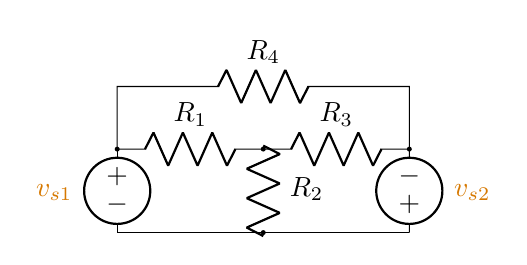
\begin{tikzpicture}[scale=0.53]
        \exM{0}{0}
      \end{tikzpicture}
    \end{column}
    \begin{column}{0.53\textwidth}
      \centering
      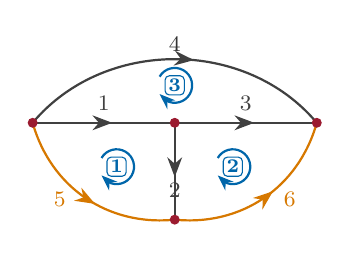
\begin{tikzpicture}[scale=0.82]
        \exMgraph{1}
      \end{tikzpicture}\\[4pt]
      {\small 1--4: $R_1, \dots, R_4$; \ \textcolor{cvolt}{5, 6: $v_{s1}$, $v_{s2}$} ($+$ to $-$)}
    \end{column}
  \end{columns}
  \vfill
  \begin{columns}[c,onlytextwidth]
    \begin{column}{0.42\textwidth}
      \small
      Mesh matrix $M$?\\[6pt]
      \onslide<2->{%
      One row per inner mesh\\[3pt]
      $+1$ along, \ $-1$ against}
    \end{column}
    \begin{column}{0.56\textwidth}
      \centering
      \only<2>{$M = \exMmatN{0}$}\only<3>{$M = \exMmatN{1}$}\only<4>{$M = \exMmatN{2}$}%
      \only<5>{$M = \exMmatN{3}$}\only<6->{$M = \exMmatN{4}$}
    \end{column}
  \end{columns}
  \vfill
\end{frame}

%--------------------------------------------------------------
\begin{frame}{$Z_M$ from the graph: KVL, KCL and Ohm's law in blocks}
  Resistors first, then voltage sources:
  \[
    M = [\,M_R \ \ M_S\,], \qquad
    \Icol{\mathbf{i}} = \begin{bmatrix} \Icol{\mathbf{i}_R}\\ \Icol{\mathbf{i}_S} \end{bmatrix}, \qquad
    \Vcol{\mathbf{v}} = \begin{bmatrix} \Vcol{\mathbf{v}_R}\\ \Vcol{\mathbf{v}_S} \end{bmatrix}
  \]
  \vfill
  \onslide<2->{%
  \textbf{KVL:} \
  $M\Vcol{\mathbf{v}} = [\,M_R \ \ M_S\,]\begin{bmatrix} \Vcol{\mathbf{v}_R}\\ \Vcol{\mathbf{v}_S} \end{bmatrix}
   = M_R\Vcol{\mathbf{v}_R} + M_S\Vcol{\mathbf{v}_S} = \mathbf{0}$}
  \vfill
  \onslide<3->{%
  \textbf{KCL:}
  \[
    \begin{bmatrix}
      \hrow{metugray!15}{\Icol{\mathbf{i}_R}}\\
      \hrow{cvolt!12}{\Icol{\mathbf{i}_S}}
    \end{bmatrix}
    =
    \begin{bmatrix}
      \hrow{metugray!15}{M_R^T}\\
      \hrow{cvolt!12}{M_S^T}
    \end{bmatrix}
    \Icol{\mathbf{i}_M}
    \qquad
    \onslide<4->{\Rightarrow\qquad
    \Icol{\mathbf{i}_R} = M_R^T\Icol{\mathbf{i}_M} \ \ \text{(resistor rows only)}}
  \]}
  \vfill
  \onslide<5->{%
  \textbf{Ohm:} \ $\Vcol{\mathbf{v}_R} = R\,\Icol{\mathbf{i}_R}$, \quad
  $R = \mathrm{diag}(R_1, \dots, R_{b_R})$}
  \vfill
\end{frame}

%--------------------------------------------------------------
\begin{frame}{$Z_M$ from the graph: the general result}
  \vfill
  Ohm and KCL into KVL:
  \[
    M_R\Vcol{\mathbf{v}_R} + M_S\Vcol{\mathbf{v}_S}
    = M_R\, R\, \underbrace{M_R^T\Icol{\mathbf{i}_M}}_{\Icol{\mathbf{i}_R}} + M_S\Vcol{\mathbf{v}_S} = \mathbf{0}
    \quad\Rightarrow\quad
    M_R\, R\, M_R^T\,\Icol{\mathbf{i}_M} = -M_S\Vcol{\mathbf{v}_S}
  \]
  \vfill
  \onslide<2->{%
  \begin{center}
    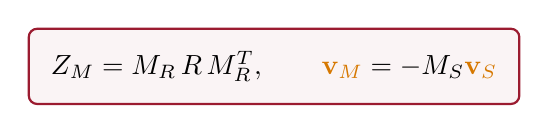
\begin{tikzpicture}
      \node[draw=metured, thick, fill=metured!5, rounded corners=3pt, inner sep=8pt]
        {$Z_M = M_R\, R\, M_R^T, \qquad \Vcol{\mathbf{v}_M} = -M_S\Vcol{\mathbf{v}_S}$};
    \end{tikzpicture}
  \end{center}}
  \vfill
  \onslide<3->{%
  \begin{center}
    $Z_M^T = M_R\, R^T M_R^T = Z_M$: \ \alert{always symmetric}
  \end{center}}
  \vfill
\end{frame}

%--------------------------------------------------------------
\begin{frame}{$Z_M$ from the graph: Example 12.1, the resistor currents}
  \begin{columns}[c,onlytextwidth]
    \begin{column}{0.36\textwidth}
      \centering
      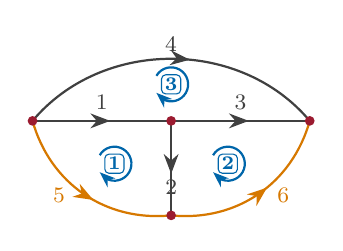
\begin{tikzpicture}[scale=0.8]
        \exMgraph{1}
      \end{tikzpicture}
    \end{column}
    \begin{column}{0.62\textwidth}
      $M_R^T$: columns 1--4 of $M$, as rows\\[8pt]
      \onslide<2->{%
      \[
        \underbrace{\begin{bmatrix}
          \Icol{i_{R_1}}\\ \Icol{i_{R_2}}\\ \Icol{i_{R_3}}\\ \Icol{i_{R_4}}
        \end{bmatrix}}_{\Icol{\mathbf{i}_R}}
        =
        \underbrace{\begin{bmatrix}
          1 & 0 & -1\\ 1 & -1 & 0\\ 0 & 1 & -1\\ 0 & 0 & 1
        \end{bmatrix}}_{M_R^T}
        \begin{bmatrix} \im{1}\\ \im{2}\\ \im{3} \end{bmatrix}
        \onslide<3->{=
        \begin{bmatrix}
          \im{1} - \im{3}\\ \im{1} - \im{2}\\ \im{2} - \im{3}\\ \im{3}
        \end{bmatrix}}
      \]}
      \onslide<4->{%
      Along minus against\\[4pt]}
      \onslide<5->{%
      Ohm: \ $\Vcol{v_{R_k}} = R_k\Icol{i_{R_k}}$}
    \end{column}
  \end{columns}
\end{frame}

%--------------------------------------------------------------
\begin{frame}{$Z_M$ from the graph: Example 12.1, the matrix}
  \vfill
  \[
    M_R\, R =
    \begin{bmatrix}
      R_1 & R_2 & 0 & 0\\
      0 & -R_2 & R_3 & 0\\
      -R_1 & 0 & -R_3 & R_4
    \end{bmatrix}
  \]
  \vfill
  \onslide<2->{%
  \[
    M_R\, R\, M_R^T =
    \begin{bmatrix}
      R_1 + R_2 & -R_2 & -R_1\\
      -R_2 & R_2 + R_3 & -R_3\\
      -R_1 & -R_3 & R_1 + R_3 + R_4
    \end{bmatrix}
    \onslide<3->{= Z_M \ \ \yes}
  \]}
  \vfill
  \onslide<4->{%
  \[
    -M_S\Vcol{\mathbf{v}_S} =
    -\begin{bmatrix} -1 & 0\\ 0 & -1\\ 0 & 0 \end{bmatrix}
    \begin{bmatrix} \Vcol{v_{s1}}\\ \Vcol{v_{s2}} \end{bmatrix}
    =
    \begin{bmatrix} \Vcol{v_{s1}}\\ \Vcol{v_{s2}}\\ 0 \end{bmatrix}
    \onslide<5->{= \Vcol{\mathbf{v}_M} \ \ \yes}
  \]}
  \vfill
  \onslide<6->{\centering The rules = this product\par}
  \vfill
\end{frame}

%==============================================================
\roadmapframe{3}

%--------------------------------------------------------------
\begin{frame}{Example 12.2: a current source on one mesh only}
  \begin{columns}[c,onlytextwidth]
    \begin{column}{0.46\textwidth}
      \centering
      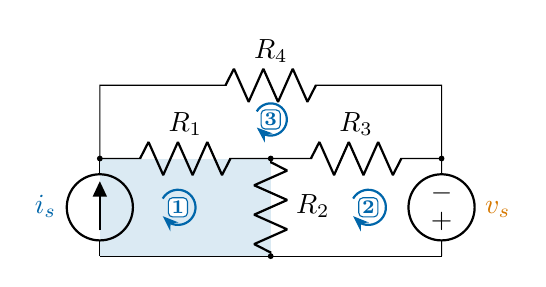
\begin{tikzpicture}[scale=0.62]
        \only<1-2>{\fill[ccur!14] (0,0) rectangle (3.5,2);}
        \exM{1}{1}
      \end{tikzpicture}
    \end{column}
    \begin{column}{0.52\textwidth}
      \small
      $\im{1} = \Icol{i_s}$: \alert{known}\\[6pt]
      \onslide<2->{%
      No KVL around mesh 1. \ Unknowns: $\im{2}$, $\im{3}$\\[10pt]}
      \onslide<3->{%
      \textbf{Mesh 2:} \
      $R_2(\im{2} - \Icol{i_s}) + R_3(\im{2} - \im{3}) - \Vcol{v_s} = 0$\\[6pt]}
      \onslide<4->{%
      \textbf{Mesh 3:} \
      $R_1(\im{3} - \Icol{i_s}) + R_3(\im{3} - \im{2}) + R_4\,\im{3} = 0$\\[10pt]}
      \onslide<5->{%
      $\begin{bmatrix}
        R_2 + R_3 & -R_3\\
        -R_3 & R_1 + R_3 + R_4
      \end{bmatrix}
      \begin{bmatrix} \im{2}\\ \im{3} \end{bmatrix}
      =
      \begin{bmatrix} \Vcol{v_s} + \alert{R_2\Icol{i_s}}\\ \alert{R_1\Icol{i_s}} \end{bmatrix}$}
    \end{column}
  \end{columns}
\end{frame}

%==============================================================
\roadmapframe{4}

%--------------------------------------------------------------
\begin{frame}{Example 12.3: a current source between two meshes}
  \vfill
  \begin{center}
    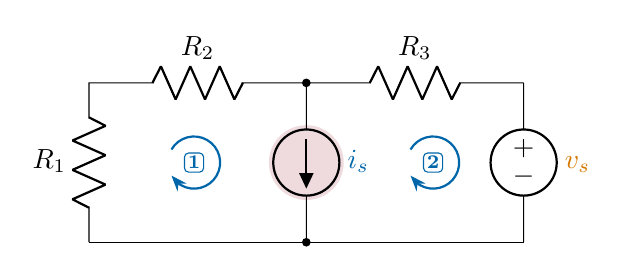
\begin{tikzpicture}[scale=0.92]
      \only<1-2>{\node[halo] at (3,1.1) {};}
      \exN{0}{1}
    \end{tikzpicture}
  \end{center}
  \vfill
  \begin{itemize}\itemsep8pt
    \item KVL around mesh 1: voltage across $\Icol{i_s}$?
    \item<2-> Not given by $\im{1}$, $\im{2}$: a current source fixes $\Icol{i}$, not $\Vcol{v}$
    \item<3-> \alert{Method I}: its voltage as an unknown \quad \alert{Method II}: supermesh
  \end{itemize}
  \vfill
\end{frame}

%--------------------------------------------------------------
\begin{frame}{Method I: the voltage as an unknown}
  \begin{center}
    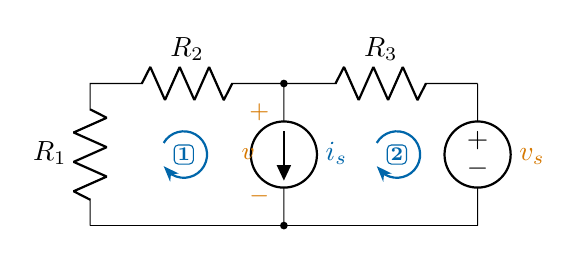
\begin{tikzpicture}[scale=0.82]
      \exN{0}{3}
    \end{tikzpicture}
  \end{center}
  \vspace{0pt}
  \begin{columns}[t,onlytextwidth]
    \begin{column}{0.58\textwidth}
      \small
      \only<-4>{%
      \onslide<2->{\textbf{Mesh 1:} \ $(R_1 + R_2)\,\im{1} + \Vcol{v} = 0$}\\[6pt]
      \onslide<3->{\textbf{Mesh 2:} \ $R_3\,\im{2} + \Vcol{v_s} - \Vcol{v} = 0$}\\[6pt]
      \onslide<4->{\textbf{Constraint:} \ $\im{1} - \im{2} = \Icol{i_s}$}}%
      \only<5->{%
      $\begin{bmatrix}
        R_1 + R_2 & 0 & 1\\
        0 & R_3 & -1\\
        1 & -1 & 0
      \end{bmatrix}
      \begin{bmatrix} \im{1}\\ \im{2}\\ \Vcol{v} \end{bmatrix}
      =
      \begin{bmatrix} 0\\ -\Vcol{v_s}\\ \Icol{i_s} \end{bmatrix}$}
    \end{column}
    \begin{column}{0.4\textwidth}
      \small
      New unknown: $\Vcol{v}$\\[6pt]
      \onslide<5->{%
      3 unknowns, 3 equations}
    \end{column}
  \end{columns}
\end{frame}

%--------------------------------------------------------------
\begin{frame}{Method II: the supermesh}
  \begin{center}
    \begin{tikzpicture}[scale=0.9]
      \only<1-2>{\exN{0}{3}}%
      \only<3->{\exN{0}{2}}%
    \end{tikzpicture}
  \end{center}
  \vspace{-4pt}
  \begin{columns}[t,onlytextwidth]
    \begin{column}{0.5\textwidth}
      Can we get rid of $\Vcol{v}$?\\[8pt]
      \onslide<2->{%
      Add KVL of meshes 1 and 2:\\[3pt]
      $\Vcol{v}$ \alert{cancels}}
    \end{column}
    \begin{column}{0.47\textwidth}
      \onslide<3->{%
      = KVL around the outer loop \nd{S}\\[6pt]}
      \onslide<4->{%
      \begin{block}{Supermesh}
        Two meshes as one, skipping the current source
      \end{block}}
    \end{column}
  \end{columns}
\end{frame}

%--------------------------------------------------------------
\begin{frame}{Method II: the equations}
  \begin{center}
    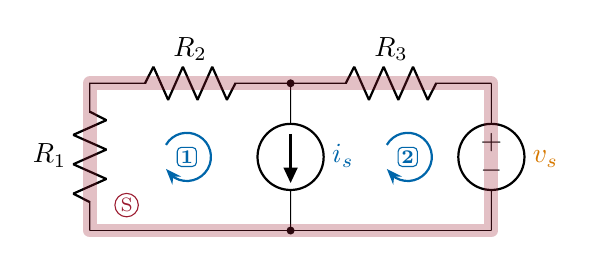
\begin{tikzpicture}[scale=0.85]
      \exN{0}{2}
    \end{tikzpicture}
  \end{center}
  \vspace{-4pt}
  \begin{columns}[t,onlytextwidth]
    \begin{column}{0.49\textwidth}
      \small
      \only<1>{KVL around the supermesh?\\[4pt]}%
      \onslide<2->{\textcolor{metured}{\textbf{Supermesh:}} \
      $(R_1 + R_2)\,\im{1} + R_3\,\im{2} + \Vcol{v_s} = 0$\\[6pt]}
      \onslide<3->{\textbf{Constraint:} \ $\im{1} - \im{2} = \Icol{i_s}$}
    \end{column}
    \begin{column}{0.49\textwidth}
      \small
      \onslide<4->{%
      \[
      \begin{bmatrix}
        R_1 + R_2 & R_3\\
        1 & -1
      \end{bmatrix}
      \begin{bmatrix} \im{1}\\ \im{2} \end{bmatrix}
      =
      \begin{bmatrix} -\Vcol{v_s}\\ \Icol{i_s} \end{bmatrix}
      \]}
      \onslide<5->{%
      2 unknowns (one fewer)\\[2pt]}
      \onslide<6->{\alert{Not} symmetric}
    \end{column}
  \end{columns}
\end{frame}

%==============================================================
\roadmapframe{6}

%--------------------------------------------------------------
\begin{frame}{Example 12.4: a dependent current source}
  \begin{columns}[c,onlytextwidth]
    \begin{column}{0.53\textwidth}
      \centering
      \begin{tikzpicture}[scale=0.68]
        \only<1-2>{\exP{0}}%
        \only<3->{\exP{1}}%
      \end{tikzpicture}
    \end{column}
    \begin{column}{0.45\textwidth}
      Find $\Icol{i}$ of the $4\ohm$.\\[10pt]
      \onslide<2->{%
      Treat $\Icol{3\,v_x}$ as a current source\\[8pt]}
      \onslide<3->{%
      Unknowns: $\im{1}$, $\im{2}$, $\im{3}$\\[8pt]}
      \onslide<4->{%
      $2\A$ between meshes 1, 2: supermesh\\[8pt]}
      \onslide<5->{%
      $\Icol{3\,v_x}$ on mesh 3 only: fixes $\im{3}$}
    \end{column}
  \end{columns}
\end{frame}

%--------------------------------------------------------------
\begin{frame}{Example 12.4: the equations}
  \begin{columns}[c,onlytextwidth]
    \begin{column}{0.53\textwidth}
      \centering
      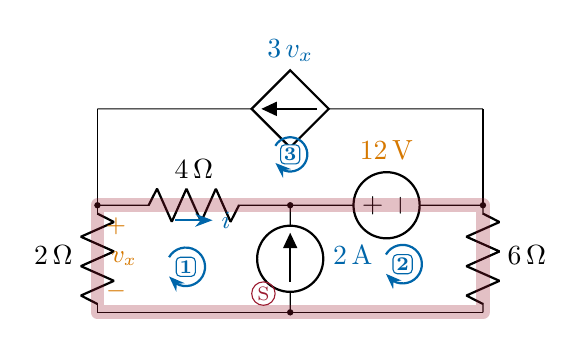
\begin{tikzpicture}[scale=0.68]
        \exP{2}
      \end{tikzpicture}
    \end{column}
    \begin{column}{0.45\textwidth}
      \small
      \only<1>{KVL around the supermesh?\\[4pt]}%
      \onslide<2->{%
      \textcolor{metured}{\textbf{Supermesh:}}\\[2pt]
      $2\,\im{1} + 4(\im{1} - \im{3}) + 12 + 6\,\im{2} = 0 \quad (1)$\\[8pt]}
      \onslide<3->{%
      \textbf{$2\A$ source:} \ $\im{2} - \im{1} = 2 \quad (2)$\\[8pt]}
      \onslide<4->{%
      \textbf{Dependent source:} \ $\im{3} = -3\,\Vcol{v_x}$\\[8pt]}
      \onslide<5->{%
      $\Vcol{v_x}$ in mesh currents?\\[4pt]}
      \onslide<6->{%
      $\Vcol{v_x} = -2\,\im{1}$\\[8pt]}
      \onslide<7->{%
      \textbf{Constraint:} \ $\im{3} = 6\,\im{1} \quad (3)$}
    \end{column}
  \end{columns}
\end{frame}

%--------------------------------------------------------------
\begin{frame}{Example 12.4: matrix form}
  \vfill
  (1), (2), (3):
  \[
    \begin{bmatrix}
      6 & 6 & -4\\[3pt]
      -1 & 1 & 0\\[3pt]
      -6 & 0 & 1
    \end{bmatrix}
    \begin{bmatrix} \im{1}\\[3pt] \im{2}\\[3pt] \im{3} \end{bmatrix}
    =
    \begin{bmatrix} -12\\[3pt] 2\\[3pt] 0 \end{bmatrix}
  \]
  \vfill
  \onslide<2->{%
  \begin{center}
    $\im{1} = 2\A$, \ $\im{2} = 4\A$, \ $\im{3} = 12\A$
  \end{center}}
  \vfill
  \onslide<3->{%
  \begin{center}
    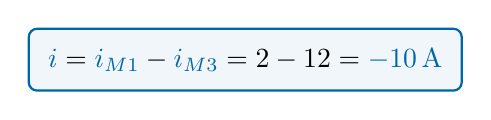
\begin{tikzpicture}
      \node[draw=ccur, thick, fill=ccur!6, rounded corners=3pt, inner sep=7pt]
        {$\Icol{i} = \im{1} - \im{3} = 2 - 12 = \Icol{-10\A}$};
    \end{tikzpicture}
  \end{center}}
  \vfill
\end{frame}

%--------------------------------------------------------------
\begin{frame}{Dependent sources}
  \vfill
  \begin{itemize}\itemsep12pt
    \item Like an independent source of the same kind
    \item<2-> Control variable in mesh currents: a \alert{constraint}
    \item<3-> Dependent \alert{voltage} source: one more term in KVL
  \end{itemize}
  \vfill
  \onslide<4->{%
  \begin{block}{Remark}
    Dependent current source on mesh $k$ only:\\[3pt]
    \alert{no} KVL around mesh $k$; write the constraint instead
  \end{block}}
  \vfill
\end{frame}

%==============================================================
\roadmapframe{7}

%--------------------------------------------------------------
\begin{frame}{Example 12.4 with node voltages}
  \begin{columns}[c,onlytextwidth]
    \begin{column}{0.53\textwidth}
      \centering
      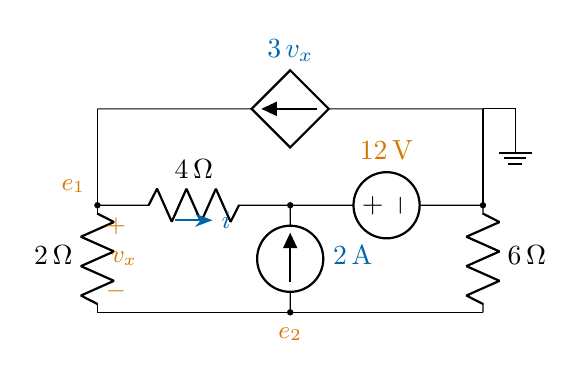
\begin{tikzpicture}[scale=0.68]
        \exP{3}
      \end{tikzpicture}
    \end{column}
    \begin{column}{0.45\textwidth}
      \small
      Same circuit, node voltages?\\[10pt]
      \onslide<2->{%
      Middle node: $12\V$ known\\[3pt]
      Unknowns: $\e{1}$, $\e{2}$\\[10pt]}
      \onslide<3->{%
      \textbf{Node 1:} \
      $\displaystyle \frac{\e{1} - \e{2}}{2} + \frac{\e{1} - 12}{4} - 3\,\Vcol{v_x} = 0$\\[6pt]}
      \onslide<4->{%
      \textbf{Node 2:} \
      $\displaystyle 2 + \frac{\e{2} - \e{1}}{2} + \frac{\e{2}}{6} = 0$\\[8pt]}
      \onslide<5->{%
      \textbf{Constraint:} \ $\Vcol{v_x} = \e{1} - \e{2}$}
    \end{column}
  \end{columns}
\end{frame}

%--------------------------------------------------------------
\begin{frame}{Example 12.4 with node voltages: matrix form}
  \vfill
  \textbf{First} plug $\Vcol{v_x} = \e{1} - \e{2}$ into node 1:
  \[
    \frac{\e{1} - \e{2}}{2} + \frac{\e{1} - 12}{4} - 3(\e{1} - \e{2}) = 0
    \onslide<2->{\qquad\Rightarrow\qquad -\tfrac94\,\e{1} + \tfrac52\,\e{2} = 3}
  \]
  \vfill
  \onslide<3->{%
  \[
    \begin{bmatrix} -\frac94 & \frac52\\[3pt] -\frac12 & \frac23 \end{bmatrix}
    \begin{bmatrix} \e{1}\\[3pt] \e{2} \end{bmatrix}
    =
    \begin{bmatrix} 3\\[3pt] -2 \end{bmatrix}
    \qquad\onslide<4->{\Rightarrow\qquad \e{1} = -28\V, \quad \e{2} = -24\V}
  \]}
  \vfill
  \onslide<5->{%
  \begin{center}
    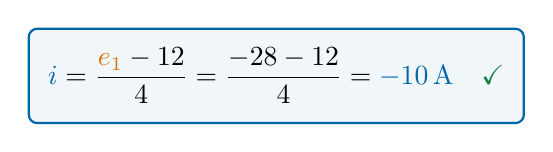
\begin{tikzpicture}
      \node[draw=ccur, thick, fill=ccur!6, rounded corners=3pt, inner sep=7pt]
        {$\displaystyle \Icol{i} = \frac{\e{1} - 12}{4} = \frac{-28 - 12}{4} = \Icol{-10\A}$ \ \ \yes};
    \end{tikzpicture}
  \end{center}}
  \vfill
\end{frame}

%--------------------------------------------------------------
\begin{frame}{Node or mesh?}
  \vfill
  Example 12.4: which needs fewer equations?
  \vfill
  \begin{columns}[t,onlytextwidth]
    \begin{column}{0.47\textwidth}
      \onslide<2->{%
      \begin{block}{Mesh currents}
        $\ell = 3$, \ 2 current sources\\[3pt]
        $3 - 2 = \alert{1}$ equation
      \end{block}}
    \end{column}
    \begin{column}{0.47\textwidth}
      \onslide<3->{%
      \begin{block}{Node voltages}
        $n - 1 = 3$, \ 1 voltage source\\[3pt]
        $3 - 1 = \alert{2}$ equations
      \end{block}}
    \end{column}
  \end{columns}
  \vfill
  \onslide<4->{%
  \begin{center}
    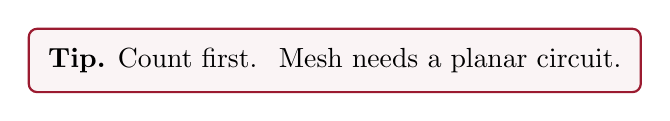
\begin{tikzpicture}
      \node[draw=metured, thick, fill=metured!5, rounded corners=3pt, inner sep=7pt, align=center]
        {\textbf{Tip.} Count first. \ Mesh needs a planar circuit.};
    \end{tikzpicture}
  \end{center}}
  \vfill
\end{frame}

%--------------------------------------------------------------
\begin{frame}{Summary}
  \vfill
  \begin{center}
  \renewcommand{\arraystretch}{1.5}
  \begin{tabular}{@{}>{\raggedright}p{4.9cm} >{\raggedright\arraybackslash}p{7.4cm}@{}}
    \toprule
    \textbf{In the circuit} & \textbf{What to do}\\
    \midrule
    resistors, voltage sources & $Z_M\Icol{\mathbf{i}_M} = \Vcol{\mathbf{v}_M}$, by the rules; symmetric\\
    current source on one mesh & $\im{k}$ known; no KVL around mesh $k$\\
    current source between meshes & Method I or supermesh, plus constraint\\
    dependent source & control in mesh currents: constraint\\
    node or mesh? & count; mesh needs planar\\
    \bottomrule
  \end{tabular}
  \end{center}
  \vfill
  \begin{center}
    Then $\Icol{\mathbf{i}} = M^T\Icol{\mathbf{i}_M}$ and the element laws
  \end{center}
  \vfill
\end{frame}

\end{document}
